\subsection{LIME settings}

\begin{figure}[ht]
    \centering
    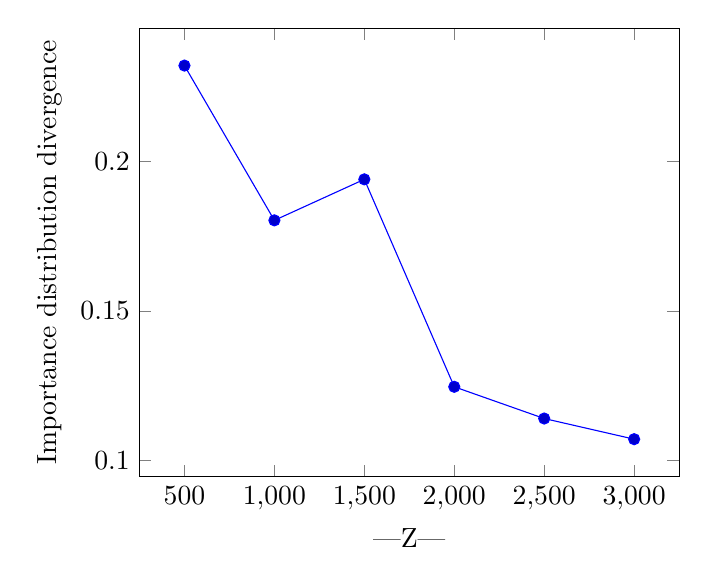
\begin{tikzpicture}
  \begin{axis}[
    xlabel={|Z|},
    ylabel={Importance distribution divergence}]
    \addplot coordinates {
      (500, 0.2320)
      (1000, 0.1803)
      (1500, 0.1940)
      (2000, 0.1247)
      (2500, 0.1141)
      (3000, 0.1072)
    };
  \end{axis}
\end{tikzpicture}

    \caption
    [Divergence of importance coefficient distributions for different numbers of input feature permutations of the Twitter data]
    {The average divergence of importance coefficient distributions across ten runs of LIME for different numbers of input feature permutations $Z$ of the Twitter data.}
    \label{fig:tweets-z}
\end{figure}
\begin{figure}[ht]
    \centering
    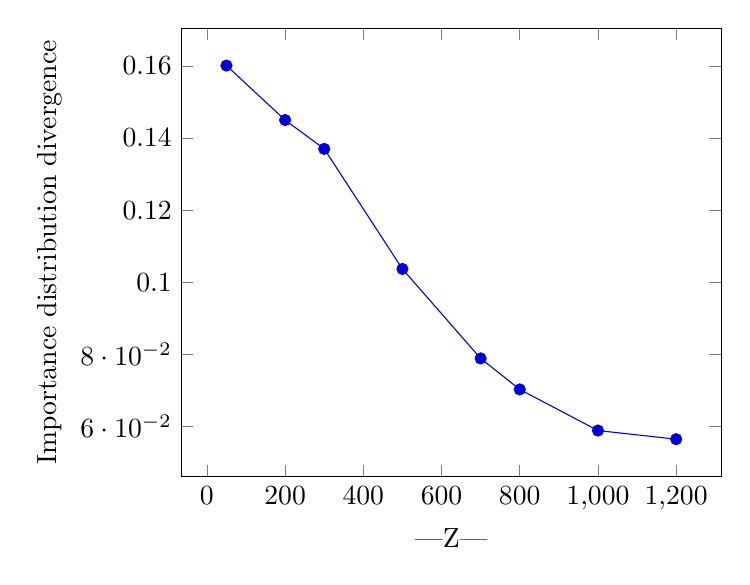
\begin{tikzpicture}
  \begin{axis}[
    xlabel={|Z|},
    ylabel={Importance distribution divergence}]
    \addplot coordinates {
      (50, 0.1601)
      (200, 0.1450)
      (300, 0.1370)
      (500, 0.1037)
      (700, 0.0789)
      (800, 0.0703)
      (1000, 0.0589)
      (1200, 0.0565)
    };
  \end{axis}
\end{tikzpicture}

    \caption
    [Divergence of importance coefficient distributions for different numbers of input feature permutations of the dialect data]
    {The average divergence of importance coefficient distributions across ten runs of LIME for different numbers of input feature permutations $Z$ of the dialect data.}
    \label{fig:dialects-z}
\end{figure}

\citeauthor{garreau2020explaining} find that, if the number of neighbourhood samples is large enough, the explanation model's feature coefficients tend to be stable across different runs of LIME. %(e.g., $\lvert{}Z\rvert=1000$) in the experiment
To generate explanations that are consistent across different runs of LIME, I experiment with varying the number of input permutations per LIME sample instance, $|Z|$.
% The more permutations are used, the more stable the results are across different initializations of LIME.

To measure the stability, I train one SVM as classification model on 90~\% of the available data and reserve the remaining instances as test data.
For each value of $|Z|$ that I test, I use the trained SVM and ten initializations of LIME to calculate global feature importance scores.
To quantify the distance between the ten resulting importance score distributions, I calculate the mean of the Jensen-Shannon distance \citep{lin1991divergence} between each (non-identical) pair of initializations.
% The Jensen-Shannon distance is defined as

% \begin{equation}
%     D_{JS}(P~\Vert~Q) = \sqrt{\frac{1}{2}D_{KL}(P~\Vert~M) + \frac{1}{2}D_{KL}(Q~\Vert~M)}
% \end{equation}

% where $M$ is the mean of $P$ and $Q$:

% \begin{equation}
%     M = \frac{1}{2}(P + Q)
% \end{equation}

% and $D_{KL}$ is the Kullback-Leibler divergence \citep{kullback1951information}:

% \begin{equation}
%     D_{KL}D(P~\Vert~Q) = \sum_{x \in X} P(x) \text{log} \frac{P(x)}{Q(x)}
% \end{equation}

As shown in \autoref{fig:tweets-z}, the divergence between importance score distributions noticeably drops when $|Z| \geq 2000$ for the Twitter data.
This also happens when $|Z| \geq 1000$ for the dialect classification task
(albeit less clearly; see \autoref{fig:dialects-z})


I set the maximum number of features with non-zero coefficients per utterance explanation, $\Omega(g_c)$, to 100.


\subsection{Representativeness and distinctiveness}
\label{sec:rep-dist}

In order to further inspect how informative a feature is, I use the measures of \textit{representativeness} and \textit{distinctiveness}, which are based on the metrics of the same name used by \citet{wieling2011bipartite} in the context of investigating features in dialectometry tasks.
\textit{Distinctiveness} is also similar to the \textit{polarized weirdness index} that \citet{poletto2020resources} use for analyzing hate speech corpora.

In the following, I define $X$ as the set of (test) input data instances, $label(x)$ as the function returning the gold standard label for a given instance of the data, and $features(x)$ as the function returning the set of explainable features contained in $x$ (which is encoded by LIME's $x'$).
\textit{Representativeness} measures the proportion of instances containing a given feature $f$ within the set of utterances that have a given gold standard label $l$:

\begin{equation}
    \text{representativeness}(f, l) = \frac{|\{x \in X~\vert~f \in \text{features}(x), \text{label(x)} = l\}|}{|\{x \in X~\vert~\text{label}(x) = l\}|}
\end{equation}

Complementarily, \textit{distinctiveness} measures the proportion of instances containing a given gold standard label $l$ within the set of utterances that have a given feature $f$, normalized by the relative size of the label class $l$:
\begin{equation}
    \text{relative-size}(l) = \frac{|\{x \in X~\text{label}(x) = l\}|}{|X|}
\end{equation}
\begin{equation}
    % spec(f, l) = \frac{|\{x \in X~\vert~f \in features(x), label(x) = l\}|}{|\{x \in X~\vert~f \in features(x)\}|}
    \text{relative-occurrence}(f, l) = \frac{|\{x \in X~\vert~f \in \text{features}(x), \text{label}(x) = l\}|}{|\{x \in X~\vert~f \in \text{features}(x)\}|}
\end{equation}
\begin{equation}
    \text{distinctiveness}(f, l) = \frac{\text{relative-occurrence}(f, l) - \text{relative-size}(l)}{1 - \text{relative-size}(l)}
\end{equation}

The highest possible distinctiveness score is 1, in which case the given feature only occurs in samples with the given label.
A distinctiveness score of 0 indicates that the feature and label co-occur as often as would be expected if they were randomly, independently distributed, i.e. they are independent of one another.
Distinctiveness has no fixed (label-independent) lower bound, but negative scores indicate that a feature and a label tend to specifically \textit{not} co-occur.

% \todo{note in discussion: comp/suff would be interesting}

% \subsection{Comprehensiveness and sufficiency}

% \todo{shorten, offer as alternative}

% \repetition{measure, degree to which}

% \cite{deyoung2020eraser} introduce several measures for determining to what extent explanations provided by machine learning models are \rephrase{faithful to ...}.
% These measures were also used in the context of detecting offensive language by \citet{mathew2020hatexplain}.
% Both measures involve selecting the features $x'_e \subseteq  x'$ that have the highest importance scores for an utterance.

% The first measure, \textit{comprehensiveness}, determines to what degree $x'_{e,c}$ contains all of the features that have a strong influence on the label prediction for the class $c$.
% Doing this involves creating a reduced representation of the utterance that only contains those features that are \textit{not} in $x'_{e,c}$, 
% % namely $\tilde{x}'_{e,c}$.
% i.e. $x' - x'_{e,c}$.
% % From this, an input representation $\tilde{x}_{e,c}$ is built to get the model's label probability for class $c$: $f(\tilde{x}_{e,c})$.
% From this, an input representation $m(x' - x'_{e,c})$ is built to get the model's label probability for class $c$: $f(m(x' - x'_{e,c}))$.
% Comprehensiveness is then defined as the difference between the probability assigned to $c$ for the original input $x$ and the reduced input:
% \begin{equation}
%     comprehensiveness(f,c,x',x'_{e,c}) = 
%     f_c(m(x'))
% %   - f_c(\tilde{x}_{e,c})
%   - f_c(m(x' - x'_{e,c}))
% \end{equation}

% Ideally, the comprehensiveness score is as close to $f_c(x)$ as possible.
% \todo{wouldn't it make more sense to scale this based on f(x). e.g. make this a ratio instead of a difference.}
% To make the comprehensiveness score meaningful for datasets with different input lengths and to take into account different potential sizes of $x'_e$, \citeauthor{deyoung2020eraser} also introduce an aggregate version of this measure.
% To do this, $|K|$ differently sized versions of $x'_{e,c}$ are constructed (and labelled $x'_{e,c,k}$ for $k \in K$).
% By default, these versions contain the top 1~\%, 5~\%, 10~\%, 20~\%, and 50~\% most important features.

% \begin{equation}
%     aggregated\text{-}comp(f,c,x',x'_{e,c},K) = \frac{1}{|K|} \sum_{k \in K} comprehensiveness(f,c,x',x'_{e,c,k})
% \end{equation}
% % NOTE: The DeYoung et al. paper is a bit ambiguous about the sum and the fraction, but their code clears this up.

% \textit{Sufficiency} on the other hand measures the degree to which $x'_{e,c}$ alone is \rephrase{sufficient} for producing a predicted label probability similar to the one the model assigns to all features in $x'$:

% \begin{equation}
%     sufficiency(f,c,x',x'_{e,c}) = 
%     f_c(m(x'))
%   - f_c(m(x'_{e,c}))
% \end{equation}

% \todo{ideal case: zero or as low as possible?}


% \todo{quote from the DeYoung paper: ``It is also computationally cheap to evaluate, in contrast to
% measures that require per-token measurements, e.g.,
% importance score correlations with ‘leave-one-out’
% scores (Jain and Wallace, 2019), or counting how
% many ‘important’ tokens need to be erased before a prediction flips (Serrano and Smith, 2019).''}